\documentclass[draft]{agujournal2019}
\usepackage{url} %this package should fix any errors with URLs in refs.
\usepackage{lineno}
\usepackage[inline]{trackchanges} %for better track changes. finalnew option will compile document with changes incorporated.
\usepackage{soul}
\linenumbers

\draftfalse

\journalname{Tectonics}


\begin{document}

\title{Laurentia's continued motion into the Neoproterozoic: new paleomagnetic constraint from the Jacobsville Formation}

\authors{Yiming Zhang\textsuperscript{1}, Blake Hodgin\textsuperscript{1}, Nicholas Swanson-Hysell\textsuperscript{1}, James Pierce\textsuperscript{1}, Anthony Fuentes\textsuperscript{1}}

\affiliation{1}{Department of Earth and Planetary Science, University of California, Berkeley, CA, USA}

\correspondingauthor{Yiming Zhang}{yimingzhang@berkeley.edu}

\begin{keypoints}
\item A new paleomagnetic pole from the ca.990 Ma Jacobsville Formation 
\item Reversals put younger bounds on the normal Keweenawan superchron 
\item The new pole indicates the Grenville Loop could be younger than thought
\end{keypoints}


\begin{abstract}
The ca. 1.1 Ga North American Midcontinent Rift resulted in protracted magmatism and the associated deposition of sediments during rift-related extension and post-rift thermal subsidence. Coeval with the cessation of rifting and a decrease of the speed of plate motion is the onset of the Grenvillian Orogeny which lasted from ca. 1090-980 Ma. The far-field stress of the orogeny is interpreted to have propagated into the interior of Laurentia and inverted the Midcontinent Rift, deforming the post-rift Jacobsville Formation whose maximum deposition age has been constrained to be ca. 990 Ma. We develop a new paleomagnetic pole from red beds of the Jacobsville Formation along 5 stratigraphic sections in Northern Michigan, USA. High-resolution thermal demagnetization experiments resolve primary magnetic remanence that pass a fold test and two conglomerate tests. Our results confirm the occurrence of geomagnetic field reversals during the deposition of Jacobsville Formation, which provides constraints for the duration of the Keweenawan superchron. Inclination corrected paleomagnetic pole position from the Jacobsville Formation confirm continued plate motion of Laurentia across the equator in the Late Mesoproterozoic to early Neoproterozoic. The new pole from the interior of Laurentia indicates the paleomagnetic poles developed from the Grenville Province may record a coherent plate motion after major continental collision during the assemblage of supercontinent Rodinia rather than recording a significant crustal shortening.
\end{abstract}

% \section*{Plain Language Summary}
% [ enter your Plain Language Summary here or delete this section]


\begin{keypoints}
\item Neoproterozoic
\item Laurentia  
\item Paleogeography
\item Inclination shallowing
\item Grenville
\item Keweenawan superchron
\item Red bed
\end{keypoints}

\section*{Introduction}

The extensively studied paleomagnetic records of the ca. 1109 Ma to 1084 Ma North American Midcontinent Rift (i.e. the Keweenawan Track) provides crucial constraints on global paleogeography in the Mesoproterozoic and has become the central record for reconstructing the development of ancient supercontinent Rodinia \cite{Swanson-Hysell2019a, Swanson-Hysell2021c}. As the rifting ceased and subsequently inverted following the onset of the Grenvillian Orogeny on Laurentia's eastern margin (Fig. \ref{fig:Geologic_map}), magmatism in the interior of Laurentia entered a quiescence period that could have lasted as much as $\sim$300 Myr until the emplacement of the ca. 780 Ma Gunbarrel large igneous province \cite{Harlan2003a}. As a result, uncertainties exist in reconstructing Laurentia and its conjugate continents' configuration in the late Mesoproterozoic to early Neoproterozoic. 

\begin{figure*}[h!]
\centering
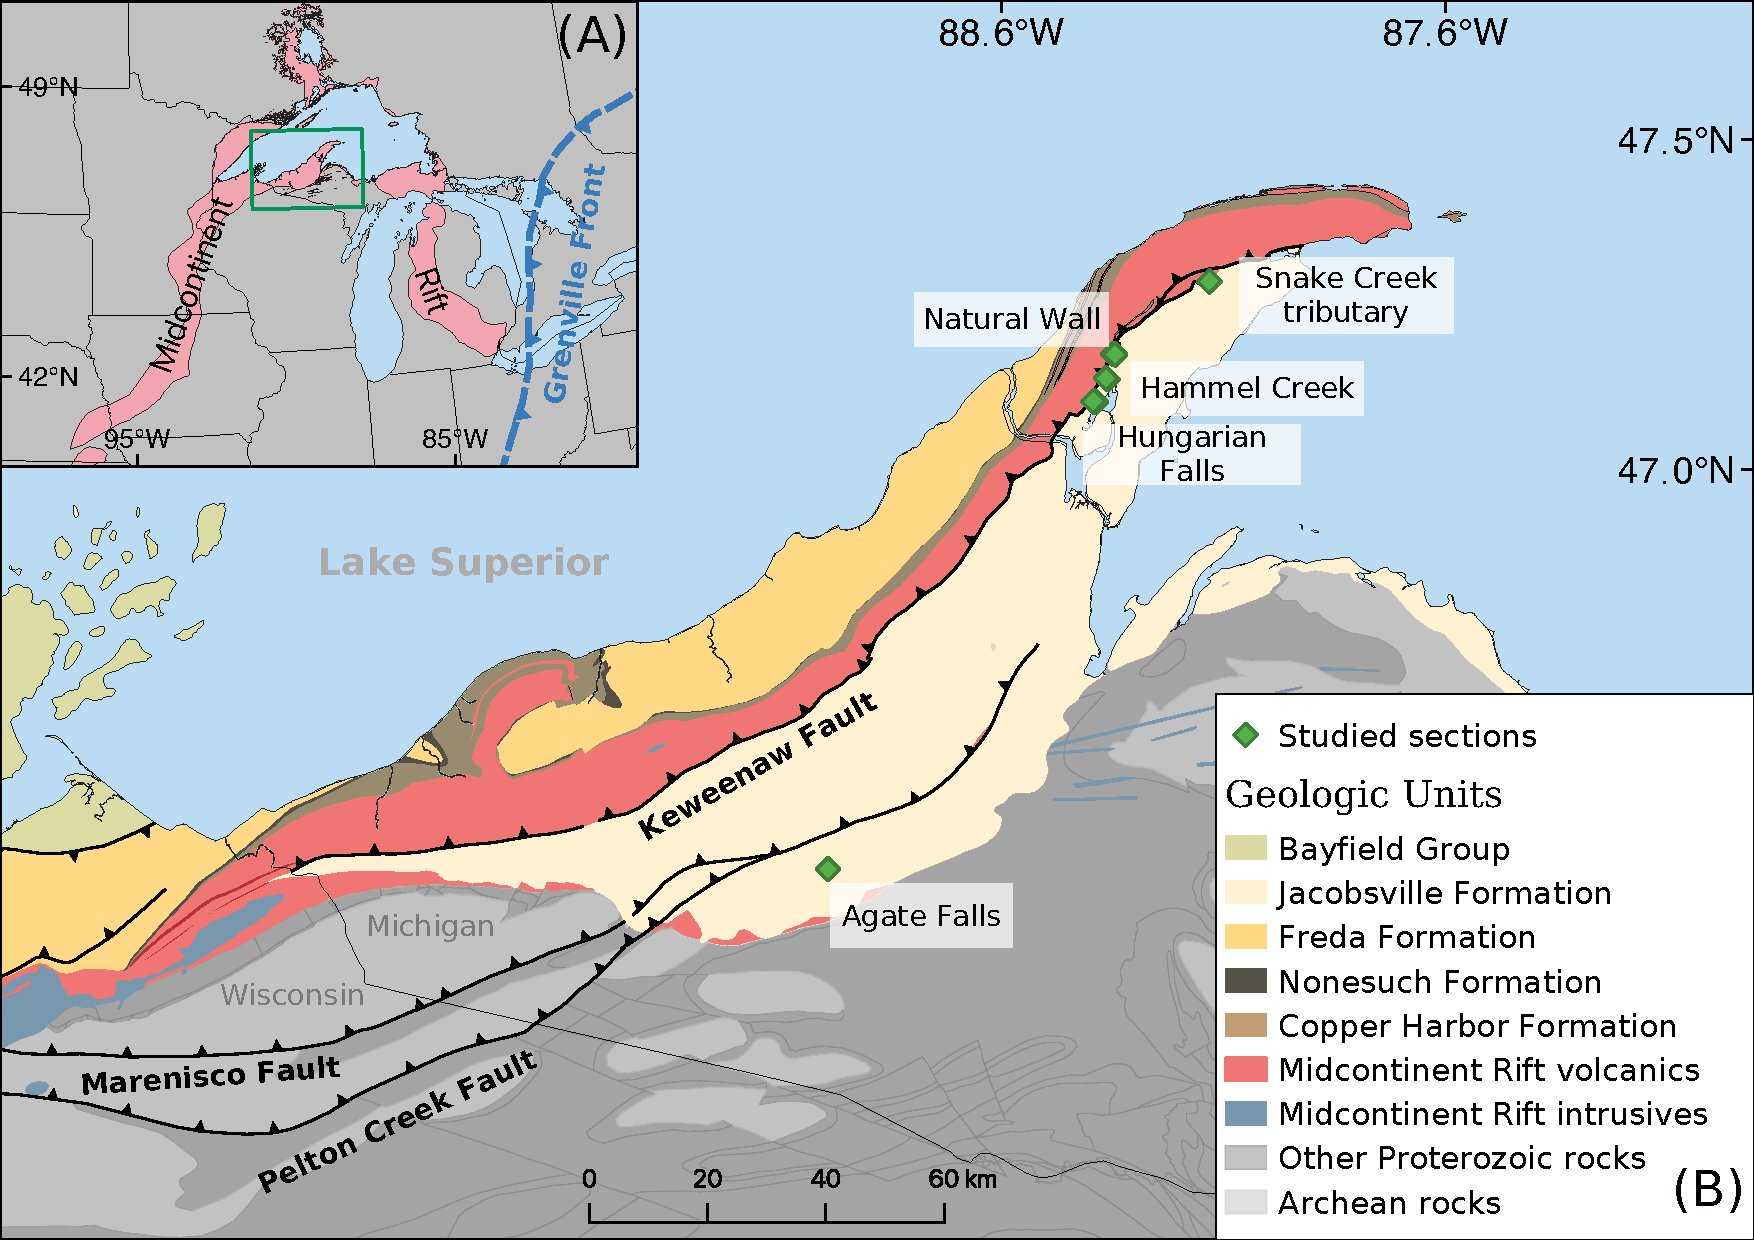
\includegraphics[width=\textwidth]{Geologic_map.pdf}
\caption{(A) Regional map showing location of the Grenville Front relative to the study area. (B) Geologic map of northern Michigan and Wisconsin showing Midcontinent Rift igneous and sedimentary rocks, the Jacobsville Formation, and major post-rift thrust faults. Jacobsville stratigraphic sections along which paleomagnetic samples were collected are shown as green diamond symbols.}
\label{fig:Geologic_map}
\end{figure*}

Although igneous activities are lacking, sedimentary rocks formed near the end of the Midcontinent Rift magmatism and afterwards, and can provide additional paleomagnetic data. In particular, hematite-bearing sedimentary rocks (i.e. red beds) can provide insights into the ancient geomagnetic field and the paleogeographic positions of sedimentary basins. In the Midcontinent Rift, the paleomagnetic poles developed from the ca. 1075 Ma Nonesuch Formation and the ca. 1070 Ma upper Freda Formation of the Oronto Group sediments that overlie the Midcontinent Rift volcanics in southern Lake Superior area (Fig. \ref{fig:Geologic_map}) provide crucial constraints for Laurentia's latitude, orientation, and plate motion in the late Mesoproterozoic \cite{Henry1977a}. 

In addition to the Oronto Group sediments, the overlying post-rift Jacobsville Formation which were deformed during the inversion of the Midcontinent Rift also contains abundant red beds which bear the opportunity to further extend the reconstruction of the apparent polar wander path of Laurentia toward more recent times \cite{Hamblin1958a, Hodgin2022a}. U-Pb detrital zircon ages and U-Pb calcite ages from late-kinematic veins constrain the maximum depositional age of the Jacobsville Formation to be ca. 990 Ma \cite{Hodgin2022a}. Developing paleomagnetic data from the Jacobsville Formation will allow further development of Laurentia's paleogeographic evolution in the late Mesoproterozoic to early Neoproterozoic. 

Challenges exist in interpreting sedimentary paleomagnetic records as they acquire magnetic remanence not through cooling from above the magnetic ordering temperatures of magnetic minerals as igneous rocks do, but acquire detrital remanence as magnetic particles settle from the water column during deposition, and chemical remanence as magnetic minerals precipitate and grow within pore spaces of host sedimentary rocks syn- to post-deposition (i.e. pigmentary hematite). It has been found that the formation of the pigmentary hematite in red beds can significantly post-date the timing of sediment deposition, resulting in the chemical remanent magnetization being secondary, superimposed upon the primary remanent magnetization carried by detrital grains \cite{Butler1992a}. To isolate the remanence components of the red beds of the Jacobsville Formation, \citeA{Roy1974, Roy1978} adopted a method first applied by \citeA{Collinson1965a} to preferentially remove fine-grained pigmentary hematite through prolonged immersion in concentrated HCl acid whereas leaving the coarser detrital grains that are more resistant to dissolution in place. Paired acid etching demagnetization and thermal demagnetization experiments show that the pigmentary hematite grains tend to have lower unblocking temperatures than detrital ones \cite{Bilardello2010a, Tauxe1980a}. High-resolution thermal demagnetization experiments with temperature intervals as small as 1-2 \textdegree C have shown to be effective in isolating detrital remanence from chemical remanence as coarser hematite grains tend to have higher unblocking temperatures \cite{Swanson-Hysell2019b}. In particular, \cite{Swanson-Hysell2019b} conducted a conglomerate test on a suite of fluvial intraclasts of the red beds in the Freda Formation to show that via thermal demagnetization one can isolate the primary magnetization (which are reoriented in random directions in the clasts) from the secondary component carried by the co-occurring authigenic hematite (which yield similar directions amongst clasts). 

Paleomagnetism of red beds has also been challenged by the controversial issue of correcting for inclination shallowing \cite{King1955a, Taux2004b, Bilardello2016b}. Due to the rotation of detrital magnetic grains toward bedding-parallel caused by authigenic processes such as compaction during lithification, inclinations recorded by sediments often have shallower angles than what was during the time of deposition. To correct for such bias, \citeA{Tauxe2004b} developed a statistical model based on the geocentric axial dipole (GAD) hypothesis where the amount of inclination shallowing in a specific sediment package is evaluated based on the shape of the distribution of the sedimentary paleomagnetic directions is compared to that predicted by a paleosecular variation model developed for the past 5 Myr. \citeA{Pierce2022a} showed that the paleosecular variation model of \citeA{Tauxe2004b} is also suitable for application to sedimentary rocks formed during the Midcontinent Rift. That study also further extended the method to better represent uncertainties associated with the amount of inclination shallowing when reporting sedimentary paleomagnetic pole positions by using the spherical elliptical Kent distribution \cite{Kent1982a} instead of the commonly used circular Fisher distribution \cite{Fisher1953a}. 

In this study, we investigate the hematite-bearing, fine-grained sandstone to siltstone lithofacies along five stratigraphic sections of the Jacobsville Formation. High-resolution thermal demagnetization data on centimeter-scale siltstone intraclasts that were eroded by fluvial processes and redeposited at two locations constrain the timing of hematite acquisition by revealing a primary component that formed prior to the erosion of the clasts within the depositional environment and a secondary component that formed following their redeposition. Then we develop a new inclination-corrected paleomagnetic pole for the Jacobsville Formation based on a large number of samples and investigate the paleo-continental configuration of Laurentia and its association with Baltica during the development of the supercontinent Rodinia. 


% preservation of the Midcontinent Rift sedimentary rocks (Figure \ref{fig:Geologic_map}), complex magnetic remanence components that often form during significantly different times within the rocks and post-deposition modification of the remanence magnetization directions are common to sedimentary rocks, presenting challenges to the interpretation of their paleomagnetic records \cite{Beck2003a, Butler1992a, Vandervoo2012a}. In contrast to igneous rocks which acquire thermal remanent magnetizations through cooling of iron oxides, red beds often record mixtures of magnetic remanence components during primary hematite grain deposition and secondary hematite precipitation and growth that are often not coeval \cite{Tauxe1980a, Swanson-Hysell2019b}. Detrital hematite grains can record magnetic remanence at the time of deposition, whose age can be constrained by the maximum deposition age of the host sedimentary rock. The secondary source of hematite is the grains that precipitate and grow in situ within pore space of host sedimentary rocks that have been deposited (i.e. pigmentary hematite). These secondary hematite could form significantly after deposition of the sedimentary rocks and can keep growing through a protracted period of time. To isolate the primary magnetization component from the secondary one within red beds is crucial for accurately reconstructing paleomagnetic records at the time of red beds deposition. Another challenge to interpreting sedimentary paleomagnetic data is the problem of inclination shallowing \cite{King1955a}. Grain rotation toward being bedding plane parallel during processes associated with deposition and lithification can result in recorded inclinations being shallower than the local magnetic inclination. Such deviation may vary depending on the location where the sedimentary rock formed and can result in various degrees of uncertainties of paleomagnetic reconstructions. 




% The end of the ca. 1109 Ma to 1084 Ma intracontinental Midcontinent Rift magmatism and extension was marked by a transition to deposition of sedimentary rocks of the Oronto Group \cite{Ojakangas2001a} as the rift basin thermally subsided prior to the rift undergoing contractional deformation in the later stages of the Grenvillian orogeny \cite{Cannon1992b, Hodgin2022a}.

%  that has become central to the reconstruction of paleogeography of the assembly of supercontinent Rodinia. In addition to syn-rift rocks preservation, the cessation and later inversion of the rift allowed the development of syn-to post-rift basin development which accommodated the deposition of the ca. 1080 - 1050 Ma Oronto Group sedimentary rocks that are in total about 5 km thick. Overlying the Oronto Group is the Jacobsville formation which has been interpreted to be deposited in a back-bulge setting associated with the far-field propagation of the crustal-scale deformation caused by the Grenvillian Orogeny.

% Previous paleomagnetic data from the Midcontinent Rift rocks that are paired with high-precision geochronology data has led to the development of the Keweenawan Track, showing rapid plate motion (latitudinal motion of $\sim$ cm/yr) from high latitudes between ca. 1105 Ma and ca. 1092 Ma, followed by a decrease in plate motion (latitudinal motion of $\sim$) between ca. 1092 Ma and ca. 1080 Ma when Laurentia moved to the equator and ceased its rapid motion. In particular, paleomagnetic poles developed from the ca. 1080 Ma Nonesuch Formation and the ca. 1050 Ma upper Freda Formation of the Oronto Group sediments indicate that Laurentia's plate speed significantly reduced in the late Mesoproterozoic, resulting in little change in its paleocontinental configuration for tens of millions of years. 

% A leading tectonic model for the cessation of the Midcontinent Rift and extension is that it occurred due to far-field compressional stress associated with the ca. 1090-980 Ma Grenvillian orogeny \cite{Cannon1992a}, when the collision of Laurentia with its conjugate margins led to the development of a back-bulge basin, accommodating the deposition of the Jacobsville Formation sediments as the inversion of the Midcontinent Rift progressed. Recent re-examination of the maximum deposition age of the Jacobsville Formation using zircon U-Pb whole grain chemical abrasion isotope dilution thermal ionization mass spectrometry has updated the maximum deposition age of the Jacobsville Formation to be ca. 990 Ma \cite{Hodgin2022a}. Such age constraint is consistent with backbulge subsidence model \cite{DeCelles, 2012}, indicating that the Jacobsville Formation may have been deposited in a Grenvillian foreland basin system that resulted from lithospheric flexure induced by orogenic loading \cite{Rivers2012a}. The relatively young age of the Jacobsville Formation compared to other Midcontinent Rift rocks makes the Jacobsville Formation an crucial target for further reconstructing the global paleogeography in the late Proterozoic. For further refining the paleogeographic connection between the poles of the Grenville Loop and those of the Keweenawan Track. 


% \cite{Roy1978a} has done that but without the effort of distinguishing the detrital remanence and the chemical rmanence.
% In addition, constraining the pole position of the 


% and shed new lights on reconciling the connection between the Keweenawan Track and the Grenville Loop paleomagnetic apparent polar wander paths. 




% Paleomagnetic data for the Jacobsville Formation have led to a paleomagnetic pole position that appears to be a continuation of the Keweenawan Track from the Oronto Group poles (Roy and Robertson, 1978; Fig. 7; Table 4). As a result, its age has been interpolated to be latest Mesoproterozoic (e.g., 1020 Ma in Li et al., 2008) such that it was deposited prior to the ca. 1000 Ma Grenville loop poles. However, this age assignment has recently been questioned on the basis of laser-ablation–inductively cou- pled plasma–mass spectrometry (LA-ICP-MS) U-Pb detrital zircon dates from Jacobsville Sandstone samples. Malone et al. (2016) interpreted a maximum depositional age of 959 ± 19 Ma based on the weighted mean of the four youngest grains from 2050 LA-ICP-MS zircon dates. A similar age was proposed on the basis of the youngest LA-ICP-MS U-Pb dates in the study of Craddock et al. (2013). This young maximum interpreted age is intriguing because it suggests the unconformity above the Freda Sandstone spans at least 100 m.y. and was followed by continued sedimentation in the region long after rift activity. Nevertheless, the paleo- magnetic pole of the Jacobsville Sandstone (Roy and Robertson, 1978) appears to extend the Keweenawan Track from the Oronto Group poles in a manner that may be more consistent with deposition of the Jacobsville Formation in the late Mesoproterozoic. Given the conflict with this inferred age, the large uncertainty of individual LA-ICP-MS dates, and the possibility of outlier dates in such a large data set, it is beneficial to interpret the age of the youngest Jacobsville zircons dated CA-ID-TIMS to obtain more precise constraints. Using CA-ID-TIMS, a recent study by Hodgin et al (2022) redefines the maximum deposition age of the Jacobsville Formation as ca. 993 Ma.



% The extensive paleomagnetic studies of the well-preserved late Mesoproterozoic to Neoproterozoic rocks of North America have provided the central record for global paleogeography reconstruction during the assembly and rearrangement of the postulated supercontinent Rodinia. Paleomagnetic studies of rocks from Laurentia have led to a series of paleomagnetic poles that form an apparent polar wander path (APWP) known as the ``Logan Loop" for the older high latitude poles at its apex that continues into the ``Keweenawan Track" of younger lower latitude poles that form a progression as the APWP heads toward the ``Grenville Loop" \citep{Swanson-Hysell2019a}. In particular, recent advances in pairing high-precision zircon U-Pb geochronology with high-quality paleomagnetic poles significantly improved the resolution of the Keweenawan Track and revealed Laurentia's rapid motion ($>$20 cm/yr) during the Midcontinent Rift magmatic activity from ca. 1110 Ma to ca. 1085 Ma \citep{Swanson-Hysell2019a}. 

% As the Midcontinent Rift magmatic activity wanes its strength and evolved into a failed intracontinental rift, Laurentia experienced a long period of magmatic quiescence in its interior, where basin subsidence dominated the rift basin. This was followed by the Grenville Orogeny, causing the the inversion of the rift along thrust belts such as the Keweenaw Fault (Fig. xxx). The lack of extensive magmatism from ca.1080 Ma to ca. 980 Ma in the Laurentia interior resulted in a significant gap (for at least 50 myr) of paleomagnetic poles between the Keweenawan Track (developed from interior Laurentia igneous and sedimentary rocks) and the Grenville Loop (poles developed from the Grenville Province rocks) (Fig. xxx; \cite{Swanson-Hysell2019a}).  

% Due to the lack of pmag records from the interior Laurentia, various hypotheses for the spatial relationship between the end of the Keweenawan Track and the Grenville Loop have been debated. One model argues for that the difference in pole locations indicates that the Grenville Province was once thousands of kilometers away from Interior Laurentia and was progressively approaching the southern margin of Laurentia in the late Mesoproterozoic \citep{Halls2015}. A corollary of this hypothesis is that there had to be a 4000 km shortening during the Grenville orogeny - colliding Amazonia-Laurentia. The other model favors that the Grenville Loop is a continuation of the Keweenawan Track - that the southerly continental drift of Laurentia continued across the equator onto the southern hemisphere from ca. 1070 Ma to ca.1000 Ma. and  approached this problem by developing data from metamorphosed dike and anorthosite and argued for Grenville  

% Paleomagnetic poles from the interior of Laurentia during the quiescence magmatism period is thus crucial for reconcile the discordant paleomagnetic poles of the Keweenawan Track and the Grenville Loop. The
% %Q: what are you using the poles from rocks that we know are from the Laurentia interior? (outside of the Grenville package?)

% This new age constraint on the Jacobsville provides crucial insight into the tectonic evolution of the Midcontinent Rift and the inversion of the extensional region into a compressional region due to the Grenville orogen. It also makes the Jacobsville sandstone a unique opportunity to investigate Laurentia's paleogeographical position at ca. 1 Ga as a long period of magmatic quiescence for $\sim$50 myr precedes Jacobsville deposition left a gap in Laurentia apparent polar wander path between the Keweenawan Track and the Grenville Loop (Fig. xxx). 

% Jacobsville sedimentation was preceded by a long period of volcanic and tectonic quiescence and cratonic stability so that bedrock surfaces became blanketed by paleosol and a surface of chemically resistant debris was dominated by quartz and iron-formation. 

% Previous paleomagnetic study on the red beds within the Jacobsville by \cite{Roy1978a} observed different components using AF, thermal, and chemical demagnetizations. Recognized dual polarities and recognized the complex remanence acquisition of red beds which lead to three isolated remanence components from the Jacobsville. However, that study did not recognize the problem of inclination shallowing and did not apply correction factor on the results. Moreover, the course demagnetization steps during thermal demagnetization would have had limited resolution for distinguishing the depositional remanent magnetization (DRM) and secondary chemical remanent magnetization (CRM) which have recently been shown to unblock over a narrow temperature window \cite{Swanson-Hysell2019b}. 

% In this study, we use fine-grained to silt-sized, hematite rich red beds from xxx sections along the Keweenaw Peninsula, Michigan with the goal of obtaining high-quality paleomagnetic pole from the jacobsville formation that is corrected for inclination shallowing problem and to investigate the connection between the Keweenawan Track and the Grenville Loop of the Laurentia APWP during the late Mesoproterozoic to the Neoproterozoic. 

\section*{Geologic settings}

\subsection*{Structure}
The ca. 1109 Ma to 1084 Ma North American Midcontinent Rift is a major intracontinental rift system that extends over 2000 km through Laurentia craton (Figure \ref{fig:Geologic_map}). However, the rifting failed to separate Laurentia into two continents. As its magmatism waned and thermal subsidence progressed in the rift basin, the $>$4 km of ca. 1080 Ma to 1050 Ma Oronto Group sediments \cite{Swanson-Hysell2019a, Fuentes2022a} were deposited conformably on top of the rift volcanics (Fig. \ref{fig:Geologic_map}; \cite{Cannon1992a}). Subsequently, the rift was inverted as the Grenvillian Orogeny commenced on the eastern margin of Laurentia (Figure \ref{fig:Geologic_map}; \citeA{Cannon1994a}), resulting in the propagation of far-field compressional stress deep into the interior of Laurentia. During the inversion, Paleoproterozoic and Archean crusts were uplifted via thrust faults such as the Marenisco fault and the Pelton Creek fault, forming the crustal-scale Montreal River monocline (Fig. \ref{fig:Geologic_map}; \cite{Cannon1993a}). The post-rift Jacobsville Formation overlies an erosional angular unconformity that developed on lithologies that were exhumed through this earlier reverse motion (Fig. \ref{fig:Geologic_map}; \citeA{Cannon1993a, Kalliokoski1982a}). The erosional contact and the development of paleosol between the Jacobsville and the underlying basement rocks is consistent with the interpretation that there was a prolonged period of sedimentation quiescence and net erosion between the formation of the Oronto Group sediments and the Jacobsville Formation. The overall extent of the Jacobsville Formation has been mapped along the lake shore of the Keweenaw Peninsula and is interpreted to extend eastward to Sault Ste Marie, Canada (Fig. \ref{fig:Geologic_map}; \citeA{Hamblin1958a}). 

% The Jacobsville Sandstone is unconformably overlain by the Cambrian Munising Formation (Hamblin, 1958).

As the far-field stress of the Grenvillian Orogeny continued to reach the interior of Laurentia, it thrusted and folded the Midcontinent Rift volcanics over the Jacobsville strata along the major Keweenaw fault which extends $\sim$250 km from the tip of the Keweenaw Peninsula in northern Michigan southeastward to a termination in northeastern Wisconsin (Fig. \ref{fig:Geologic_map}; \citeA{Cannon1996a, Cannon2001a, DeGraff2022a}). As a result, rift volcanic clasts where eroded into the Jacobsville basin at the same time when sediments from the older basement rocks along with distal input from the Grenville Province were deposited within the Jacobsville back-bulge basin system that in general wedges toward the northwest (Figure \ref{fig:Geologic_map}; \cite{Hedgman2014a, Hodgin2022a}. Immediately near the Keweenaw fault in the footwall, folding has also been recorded by strata of the upper Jacobsville Formation in contact with the volcanics \cite{Cannon1993a}. One famous remanence of that late-stage deformation is the Natural Wall ravine where sub-vertical to overturned sandstone beds are preserved (Figure \ref{fig:Geologic_map}; \cite{Hamblin1958a}). On shore of Bete Grise Bay near the northeastern edge of the Keweenaw Peninsula, the Keweenaw fault is interpreted to have accommodated compressional stresses by forming a series of segmented en echelon thrusts \cite{Tyrrell2019a}. The timing of such en echelon faulting could be coeval with the deposition of the upper Jacobsville Formation, leading to the nonconformable onlapping of the Jacobsville sediments over the volcanics in addition to the thrust faulting relationship between the two units. Late-kinematic calcite that precipitated within the brecciated Keweenaw fault zone and youngest detrital zircons of the Jacobsville Formation constrain the timing of the final inversion of the Keweenaw Fault to be during the Rigolet phase of the Grenvillian Orogeny \cite{Hodgin2022a}. 

\subsection{General stratigraphy}

% It has been interpreted that the Jacobsville Sandstone is equivalent to the Bayfield Group in northern Wisconsin, and the Fond Du Lac and Hinckley formations in Minnesota. Their shared lithofacies of basal conglomerate, cross-bedded fluvial fine to medium grained sandstone, and interbedded red micaceous siltstone could support the interpretation that these sedimentary rocks formed during a common period of post-rift basin formation following rift-related magmatism of the Midcontinent Rift. 
\begin{figure*}[h!]
\centering
\includegraphics[width=0.9\textwidth]{Field_photo.png}
\caption{\scriptsize Field photos of red beds of the Jacobsville Formation sampled in this study. At Baby Snake Creek and the Natural Wall ravine in northern Keweenaw Peninsula, intervals of red fine-grained sandstone beds can be found through the steeply dipping to overturned basal strata near the Keweenaw Fault (A,C) and also the nearly horizontal top strata (B,D). At Hungarian Falls, relatively thick intervals of fine-grained red sandstone to siltstone beds separated by hematite-depleted arenite to arkosic sandstones or conglomerates are found along a $\sim$100-meter-tall waterfall (E). Abundant reoriented siltstone rip-up clasts often exist within the conglomeratic layers above siltstone beds (F). Drill cores or block samples of these rip-up clasts are sampled for the paleomagnetic conglomerate test presented in Fig. \ref{fig:Intraclast_pmag}. At Agate Falls, nearly flat-lying red fissile shale beds are exposed due to waterfall incision (G). Subrounded detrital mica grains deposited parallel to the bedding plane are often associated with the siltstone facies. Another set of siltstone rip-up clasts were sampled from a conglomeratic layer near the basal exposure for the paleomagnetic conglomerate test. }
\label{fig:Field_photo}
\end{figure*}

The Jacobsville Formation is a fluvial sequence of feldspathic and quartzose sandstones, conglomerates, siltstones, and shales, completely devoid of lava flows or cross-cutting dikes. It is in general more quartz-rich than the Oronto Group sediments. Abundant near the bottom section in the southern exposures of the Jacobsville Formation, conglomerate facies typically have provenance sourced from Paleoproterozoic lithologies such as vein quartz and iron formation clasts \cite{Hamblin1958a, Kalliokoski1982a}. The occurrence of these conglomerates in proximity to the Keweenaw, Marenisco, and Pelton Creek thrust faults is interpreted to represent syn-depositional development of local relief \cite{Kalliokoski1982a, Hedgman1992a}). 

Near the Keweenaw Fault (Fig. \ref{fig:Geologic_map}), the Jacobsville Formation consists dominantly of quartz-rich, cross-bedded, medium-grained sandstone, locally abundant clast-supported conglomerate, with interbeds of hematite-bearing micaceous siltstone (Fig. \ref{fig:strat_column}). In this region, the conglomerate contains abundant volcanic clasts likely derived from uplifted Midcontinent Rift volcanics \cite{Irving1885a, Brojanigo1984a}. Occurrence of red siltstone beds have been reported in the Jacobsville Formation, particularly in the upper sections near Keweenaw Fault \cite<e.g.>{Hamblin1958a, Irving1885a}. In the field, they typically appear brick-red to dark-red, consisting of find-grained arenite to arkosic sandstone and siltstone sometimes with minor grey reduction spots (Fig. \ref{fig:Field_photo}). Rounded detrital mica grains up to $\sim$5mm in size can be found commonly within very fine, fissile siltstone and shaly strata (Figure \ref{fig:Field_photo}). The fact that in the Jacobsville has conglomerate and sandstone and siltstone facies in them supports sediment input from the eroded Oronto Group. This indicate the older boundary of the Jacobsville deposition might be closer to the Rigolet Phase than the Ottawan phase and the duration of Jacobsville sedimentation may be within a relatively constrained period of time. 


tyrrell 2019 fig. 10 recorded onlapping of the Jacobsville Formation on to the Portage Lake Volcanics which appears to have been faulted prior to the deposition of Jacobsville near Bete Grise Bay. 

% Hematite is one of the most stable form of iron oxides under ambient conditions, and magnetic remanence carried by the grains within red beds can be preserved for billions of years \cite{Butler1992a, Jiang2022a}. Previously, paleomagnetic records of the Jacobsville Formation have been investigated by \citeA{Roy1978a} who sampled a range of lithofacies of the Jacobsville Formation and obtained that a primary remanence component can be isolated via magnetic cleaning. In this study, we target the find-grained sandstone to siltstone facies in the upper Jacobsville Formation and segregate the primary and secondary remanent magnetizations using high-resolution thermal demagnetization method \cite{Swanson-Hysell2019b}. We update the paleomagnetic records of the Jacobsville Formation with additional evaluation for the degree inclination shallowing that \citeA{Roy1978a} did not take into account. 



% Along the south shore of Lake Superior, the Keweenawan Supergroup overlies Paleoproterozoic basement and consists of ~5 km of rift-related volcanic rocks that are conformably overlain by ~4 km of conglomerate, siltstone, and sandstone of the Oronto Group (Cannon et al., 1996). The uppermost unit of the Keweenawan Supergroup is the Jacobsville Sandstone, which consists of up to ~1 km of fluvial deposits that are more quartz-rich than the Oronto Group (Fig. 1; Kalliokoski, 1982). The Jacobsville Sandstone unconformably overlies Archean and Paleoproterozoic basement as well as Midcontinent Rift volcanic and sedimentary rocks in northern Michigan (Fig. 1; Cannon et al., 1993; Ojakangas et al., 2001). 

% The Keweenaw Fault is a north to northwest-dipping thrust that  Thrust faults parallel to the Keweenaw Fault include the northwest-dipping Marenisco and Pelton Creek faults (Fig. 1). Similarly-oriented thrusts continue southwestward through northern Wisconsin and eastern Minnesota (Ojakangas et al., 2001), and eastward below Lake Superior, where they are interpreted to join mapped thrust faults in southern Ontario (Fig. 1; Manson and Halls, 1994; Ojakangas et al., 2001). Rock units adjacent to these regional thrusts have been moderately to intensely folded. 

% In northern Michigan, the typically shallowly-dipping Jacobsville Sandstone has sub-vertical to overturned beds in the immediate footwall of the Keweenaw Fault (Irving and Chamberlin, 1885; Cannon and Nicholson, 2001). 




\begin{figure*}[h!]
\centering
\includegraphics[width=0.9\textwidth]{strat_column.png}
\caption{}
\label{fig:strat_column}
\end{figure*}

Keweenaw Fault motion post dating Jacobsville in the footwall
Youngest DZ from jacobsvill eis about 993 Ma (sandstone creek, about a few hundred meters from the fault). 
directly above pmag sampling at Agate falls grain B geochron date is (z2, s226, about 1000 Ma grain)

jacobsville (985.5 from calcite in the fault and <993 from zircons) 

Blake's current tectonic model: after MCR volcanics ca. 1084 Ma emplacement follows the deposition of the sediments (Oronto Group) copper harbor conglomerate, Nonesuch formation and the Freda formation. Then the Grenville orogenesis took off with the Ottawan phase from 1020 Ma - 10?? Ma and the Rigolet phase from 995-980 Ma. Paleosol development and the unconformity between the Jacobsville and the volcanics indicate a prolonged period of gap during which the Oronto Group in the backbulge basin where they were deposited were lost, resulting in younger Jacobsville deposition directly on top of the volcanics. The fact that in the Jacobsville has conglomerate and sandstone and siltstone facies in them supports sediment input from the eroded Oronto Group. This indicate the older boundary of the Jacobsville deposition might be closer to the Rigolet Phase than the Ottawan phase. The younger age boundary of the Jacobsville is well defined - given that the maximum deposition age from the zircons of the Jacobsville is 993 Ma and the calcite on the Keweenaw Fault is 985.5 Ma, the deposition of at least the upper portion of the Jacobsville is well constrained to be between 993 and 985 Ma. The deposition of Jacobsville in the back bulge in Laurentia interior is related to the far-field compression caused by the Grenville Orogeny. 

This makes the Jacobsville sandstone one unique opportunity to acquire a paleomagnetic pole position within the gap between the 



\section*{Paleomagnetic methods and results}

Oriented paleomagnetic samples were collected with a portable electric drill along five stratigraphic sections of the Jacobsville Formation in norther Michigan (Fig. \ref{fig:Geologic_map}). Additional oriented cores and block samples of siltstone rip-up clasts within conglomerate facies were sampled at Hungarian Falls and at Agate Falls. In order to maximize sampling of paleosecular variation, we optimized for vertical stratigraphic coverage and collected one sample at each red bed horizon. As such, each sample constitutes a paleomagnetic site considering that a paleomagnetic site (which ideally captures a single snapshot of the local geomagnetic field) is a particular bed in a sedimentary sequence. Red fine-grained sandstone to shale layers were preferentially sampled as they have lower permeability and are less susceptible to diagenetic alteration through fluid flow than coarser grained sandstone. Care was taken to avoid samples containing reduction spots. Paleomagnetic samples were oriented using a magnetic compass and a sun compass whenever possible. Sun compass data were preferentially used when available. A total of 379 specimens including 30 intraclasts where collected for paleomagnetic study. The specimens underwent stepwise thermal demagnetization in the UC Berkeley Paleomagnetism Lab using an ASC demagnetizer (residual fields $<$10 nT) with measurements made on a 2G DC-SQUID magnetometer. The demagnetization protocol had high-resolution approaching the Ne\'el temperature of hematite (5 \textdegree C to 2 \textdegreeC) (Fig. \ref{fig:Intraclast_pmag}). All paleomagnetic data are available to the measurement level in the MagIC database (https://earthref.org/ MagIC/; THIS LINK IS AVAILABLE TO REVIEWERS AND WILL BE UPDATED WHEN A DOI IS AVAILABLE).


\subsection*{Fluvial intraclast conglomerate test}

Similar to the thermal demagnetization result of the hematite-bearing fluvial intraclasts of the Freda Formation \cite{Swanson-Hysell2019b}, the siltstone rip-up clasts of the Jacobsville Formation also typically reveal two distinct magnetization directions (Fig. \ref{fig:Intraclast_pmag}). One direction was similar throughout the intraclasts and was typically removed up to 640-655 \textdegree C (Fig. \ref{fig:Intraclast_pmag}). This component is directionally well-grouped amongst the reoriented intraclasts, indicating that it is likely a chemical remanent magnetization acquired through the growth of secondary hematite grains following redeposition of the clasts (Fig. \ref{fig:Intraclast_pmag}). After the removal of the mid-temperature component, further thermal demagnetization with small step increments at higher temperatures up to $\sim$689 \textdegree C often reveal an origin-trending component (Fig. \ref{fig:Intraclast_pmag}). In the data from the clasts, there is typically a significant directional change in the specimen magnetization between the mid-temperature component and the high-temperature component and as a result, 28 out of 30 intraclast specimens could be fit with distinct mid-temperature and high-temperature least squares lines \cite{Kirschvink1980a}. Distinct from the well-grouped mid-temperature component directions, the high-temperature directions of the intraclasts are dispersed and the null hypothesis of randomness cannot be rejected at the 95\% confidence level (n=6 for intraclasts at Agate Falls and n=22 for intraclasts at Hungarian Falls; Fig. \ref{fig:Intraclast_pmag}; \citeA{Watson1956a}). This indicates that the component was likely acquired by the detrital hematite grains during initial formation of the clasts prior to erosion and redeposition. 


\begin{figure*}[h!]
\centering
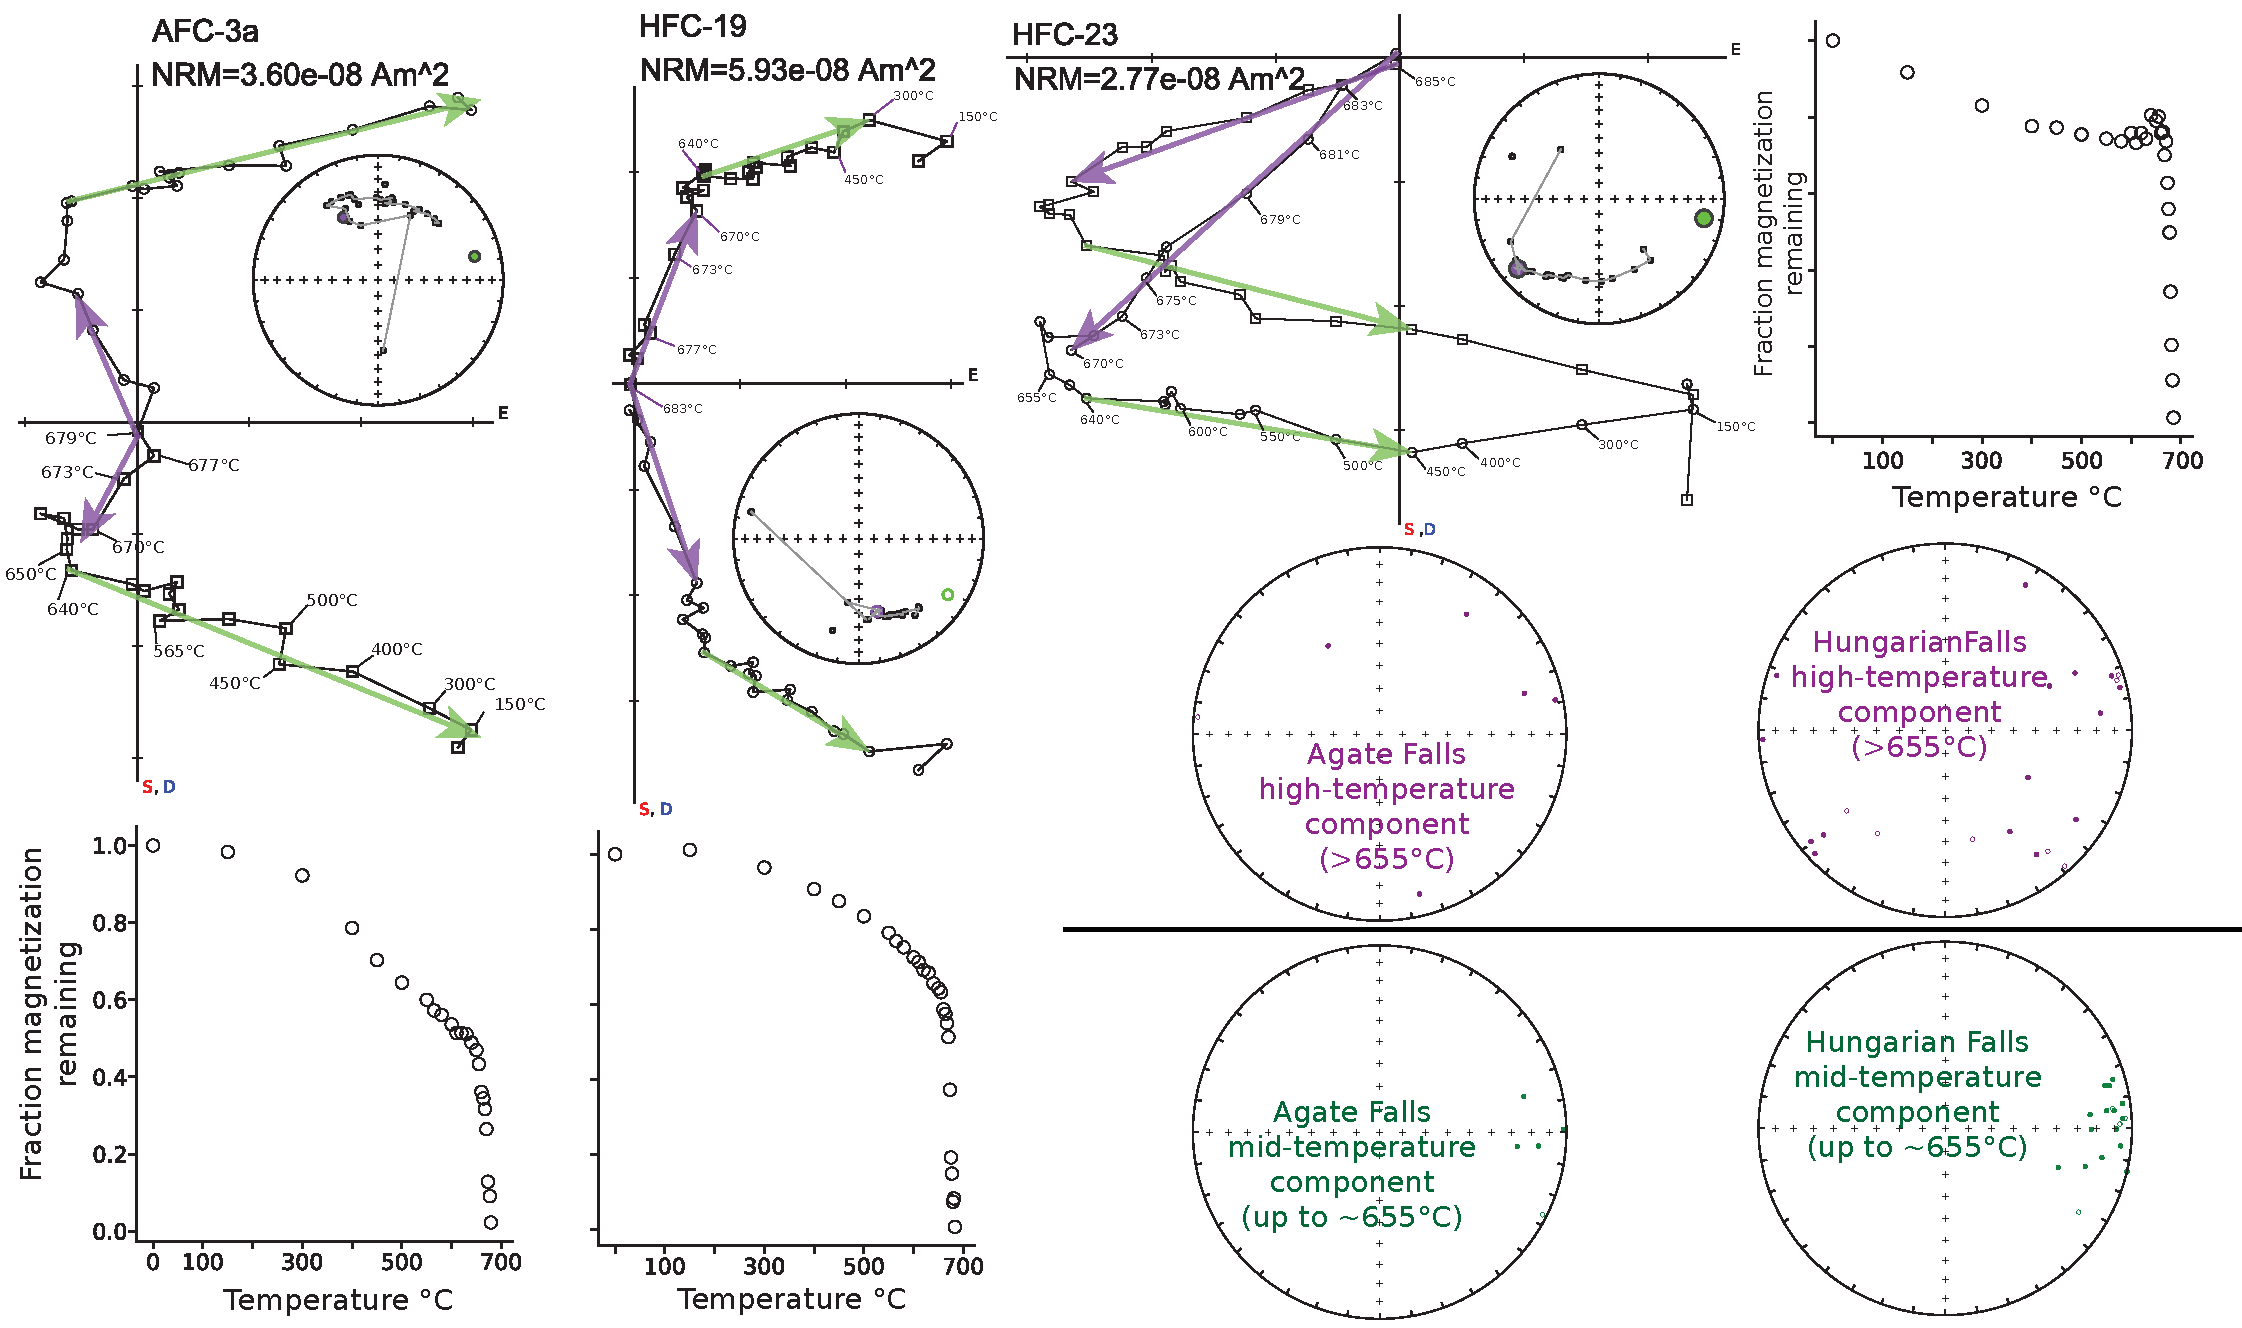
\includegraphics[width=\textwidth]{Intraclast_pmag.pdf}
\caption{Paleomagnetic data from intraclasts of the Jacobsville Formation reveal a mid-temperature component that typically unblocks prior to 655 \textdegree C and a high-temperature component that typically unblocks up to 687 \textdegree C. These components are present as varying fractions of the overall remanence as seen in the three individual clasts shown here on vector orthogonal plots and measurement-level equal area plots in tilt-corrected coordinates (developed using PmagPy; \citeA{Tauxe2016a}). The direction of the mid-temperature component is shown as green arrows on the vector component plots and green circles on the equal area plots, while the high-temperature component is shown with purple symbols. The mid-temperature component has a similar direction among the clasts as can be seen on the component directions equal area plots. In contrast, the high-temperature component directions (purple) are dispersed. NRM = natural remanent magnetization; AFC = Agate Falls clasts; HFC = Hungarian Falls clasts.}
\label{fig:Intraclast_pmag}
\end{figure*}

\subsection*{Tentative magnetostratigraphy}

With the insights gained from the thermal demagnetization results of the Jacobsville fluvial intraclasts, we next isolate the high-temperature magnetization component from the mid-temperature component for all in situ specimens that were collected along the five localities in northern Michigan (Fig. \ref{fig:Geologic_map}). The resultant high-temperature component directions are plotted by locality in Fig. \ref{fig:in_situ_pmag}. These results show dual polarities recorded by the Jacobsville Formation (Fig. \ref{fig:in_situ_pmag}), consistent with the observation of \citeA{Roy1978a}. Furthermore, our new data show that the Jacobsville Formation recorded more than one geomagnetic field polarity reversal and a tentative magnetostratigraphy may be constructed (Fig. \ref{fig:in_situ_pmag}). 

At Agate Falls (Fig. \ref{fig:Geologic_map}), multiple hematite-rich, detrital mica-bearing siltstone layers occur through a $\sim$30-meter strata incised by the running Middle Branch Ontonagon River. 68 paleomagnetic samples were collected on both sides of the river through overlapping stratigraphic sections (Fig. \ref{fig:strat_column}). A single transition from normal to reversed polarity is observed through the sections from bottom to top with a few strata in the middle of the section capturing transitional field directions (Fig. \ref{fig:strat_column}, \ref{fig:in_situ_pmag}). 

At Hungarian Falls (Fig. \ref{fig:Geologic_map}), high-energy fluvial environment led to the deposition of numerous hematite-rich siltstone to fine-grained sandstone layers, capturing richer information of the geomagnetic field variations than at other localities (Fig. \ref{fig:strat_column}). Throughout $\sim$240 meters of stratigraphy, a total of 158 samples were collected for paleomagnetic study. At stratigraphic height of $\sim$24 meters (Fig. \ref{fig:strat_column}), 8 samples from a $\sim$0.5-meter-thick siltstone layer record a reversed polarity (easterly declination and shallow inclination; horizon HF6). At stratigraphic level $\sim$42 meters (HF5; Fig. \ref{fig:strat_column}), 4 samples were collected through a $\sim$0.2 m siltstone horizon including one specimen from near the base of the layer and three specimens near the top of the layer. The high-temperature remanence component from the three specimens near the top all record a reversed polarity whereas the specimen collected near the base show a westerly declination. While more samples are needed to test whether the westerly declination recorded by the single sample is a result of the geomagnetic field having completely flipped polarity from that recorded by horizon HF6 or a result of transient unstable field, this anomalous direction indicates that the geomagnetic field did not stay consistent throughout the time of deposition of this horizon. As a result, we tentatively mark a period of transitional field near the base of horizon HF5 in Fig. \ref{fig:strat_column}. A reversed polarity field seems to have been maintained as 5 samples from horizon HF4 consistently record easterly directions similar to those recorded by samples near the top of HF5 (Fig. \ref{fig:strat_column}). However, a geomagnetic field polarity reversal happened between the deposition of siltstone layers of HF4 and HF3, as 7 samples from HF3 all record normal-polarity directions, antipodal to those of samples of HF4. Subsequently, the field appears to flip again back to reversed polarity, as is shown by 7 samples from HF2 higher above the section (Fig. \ref{fig:strat_column}). Through the $\sim$35-meter-thick horizon of HF1 characterized by numerous siltstone to fine-grained sandstone layers interbedded with coarser-grained sandstone and conglomerate, magnetic polarity reversals of R-N-R-N-R were recorded (Fig. \ref{fig:strat_column}). 

The Natural Wall ravine and Hammel Creek are of close proximity from Hungarian Falls (Fig. \ref{fig:Geologic_map}) and the sedimentary facies characterized by trough cross-bedded sandstone and conglomerates are similar to the basal $\sim$120 meter of the section at Hungarian Falls (Fig. \ref{fig:strat_column}). Since only a couple of siltstone to fine-grained sandstone horizons were sampled at these two localities, we tentatively correlate the stratigraphic sections at these three localities based on their sedimentary facies and magnetic polarities (Fig. \ref{fig:strat_column}). At Hammel Creek, 14 samples from two siltstone layers near the base of the section are of reversed polarities, consistent with the reversed-polarity layers near the base of Hungarian Falls. Near the top of the Natural Wall section, consistent normal-polarity directions are recorded by 15 samples. This normal polarity could be coeval with one of the normal-polarity periods recorded at Hungarian Falls, or it could indicate an additional polarity reversal from reversed to normal polarity that happened after the deposition of the youngest reversed strata at Hungarian Falls (Fig. \ref{fig:strat_column}). Near the base of the stratigraphic section at Natural Wall (Fig. \ref{fig:strat_column}), the strata are steeply tilted or overturned (Fig. \ref{fig:Field_photo}). Tilt-corrected paleomagnetic directions from samples collected from these strata show dominantly southeasterly declinations that are distinct from either normal- or reversed-polarity directions higher along the strata or at Hungarian Falls. Possible causes of such distinct directions could be related to transitional fields associated with geomagnetic field polarity reversals or complications in the tilt correction such as noncylindrical folding or multiple tilting episodes. 

A total of 70 specimens yielded interpretable high-temperature paleomagnetic remanence component throughout the stratigraphic section at Baby Snake Creek (Fig. \ref{fig:Geologic_map}, \ref{fig:in_situ_pmag}). The remanence directions recorded by red beds within the steeply folded basal section and within the flat-lying top portion of the section pass a bootstrap fold test (Supporting Information; \citeA{Tauxe1994a}). The remanence directions are all of normal polarity and show a dominantly southwest declination and upward-pointing inclination (Fig. \ref{fig:in_situ_pmag}). 

Given that multiple geomagnetic field reversals occurred during the deposition of the Jacobsville Formation, it is desirable that a magnetostratigraphy be developed. However, challenges exist in correlating the stratigraphic sections measured at the five localities in this study due to the lateral variability of the paleodepositional environment associated with the variable paleotopographic relief of the Precambrian surface upon which the Jacobsville Formation was deposited \cite{Hamblin1958a, Kalliokoski1982a}. In particular, there may not be a unique solution in reconstructing the relative stratigraphic positions of the strata at Baby Snake Creek and Agate Falls with respect to the other three sections in central Keweenaw Peninsula due to geographical separations (Fig. \ref{fig:Geologic_map}, \ref{fig:strat_column}). However, at both Baby Snake Creek and Agate Falls, the sedimentary strata are dominated by siltstone to cross-bedded sandstone and are lacking significant amount of conglomerate facies as seen near Hungarian Falls. This could be consistent with the interpretation that these strata were deposited as the Jacobsville basin of the Grenvillian foreland system resulted from lithospheric flexure induced by orogenic loading has been partially filled. Recent geologic mapping efforts near Baby Snake Creek have found evidence for the Jacobsville Formation onlapping the Midcontinent Rift volcanics that were previously faulted via en echelon segments\cite{Tyrrell2019a, Mueller2021a}. The unconformable contact between the sediments and the volcanics, instead of faulted contact typically observed near Hungarian Falls where the basal Jacobsville Formation is folded and faulted against the volcanics, indicate that the deposition of the Jacobsville Formation near the northern end of Keweenaw Peninsula likely post-date some episodes of motion along the Keweenaw Fault. Therefore, we interpret that the normal-polarity strata at Baby Snake Creek could be stratigraphically the youngest amongst the five localities, although a possibility that they instead are near the bottom of the stratigraphy and record the normal Keweenawan Superchron cannot be ruled out \cite{Driscoll2016b}. 

Overall, the multiple geomagnetic field polarity reversals recorded by the Jacobsville Formation constrain the maximum range of the Keweenawan normal superchron \cite{Driscoll2016b} to be between ca. 1100 (Mamainse Point Volcanics; \cite{Swanson-Hysell2019a}) to ca. 992 Ma (maximum deposition age of Jacobsville Formation; \cite{Hodgin2022a}). 


\begin{figure*}[h!]
\centering
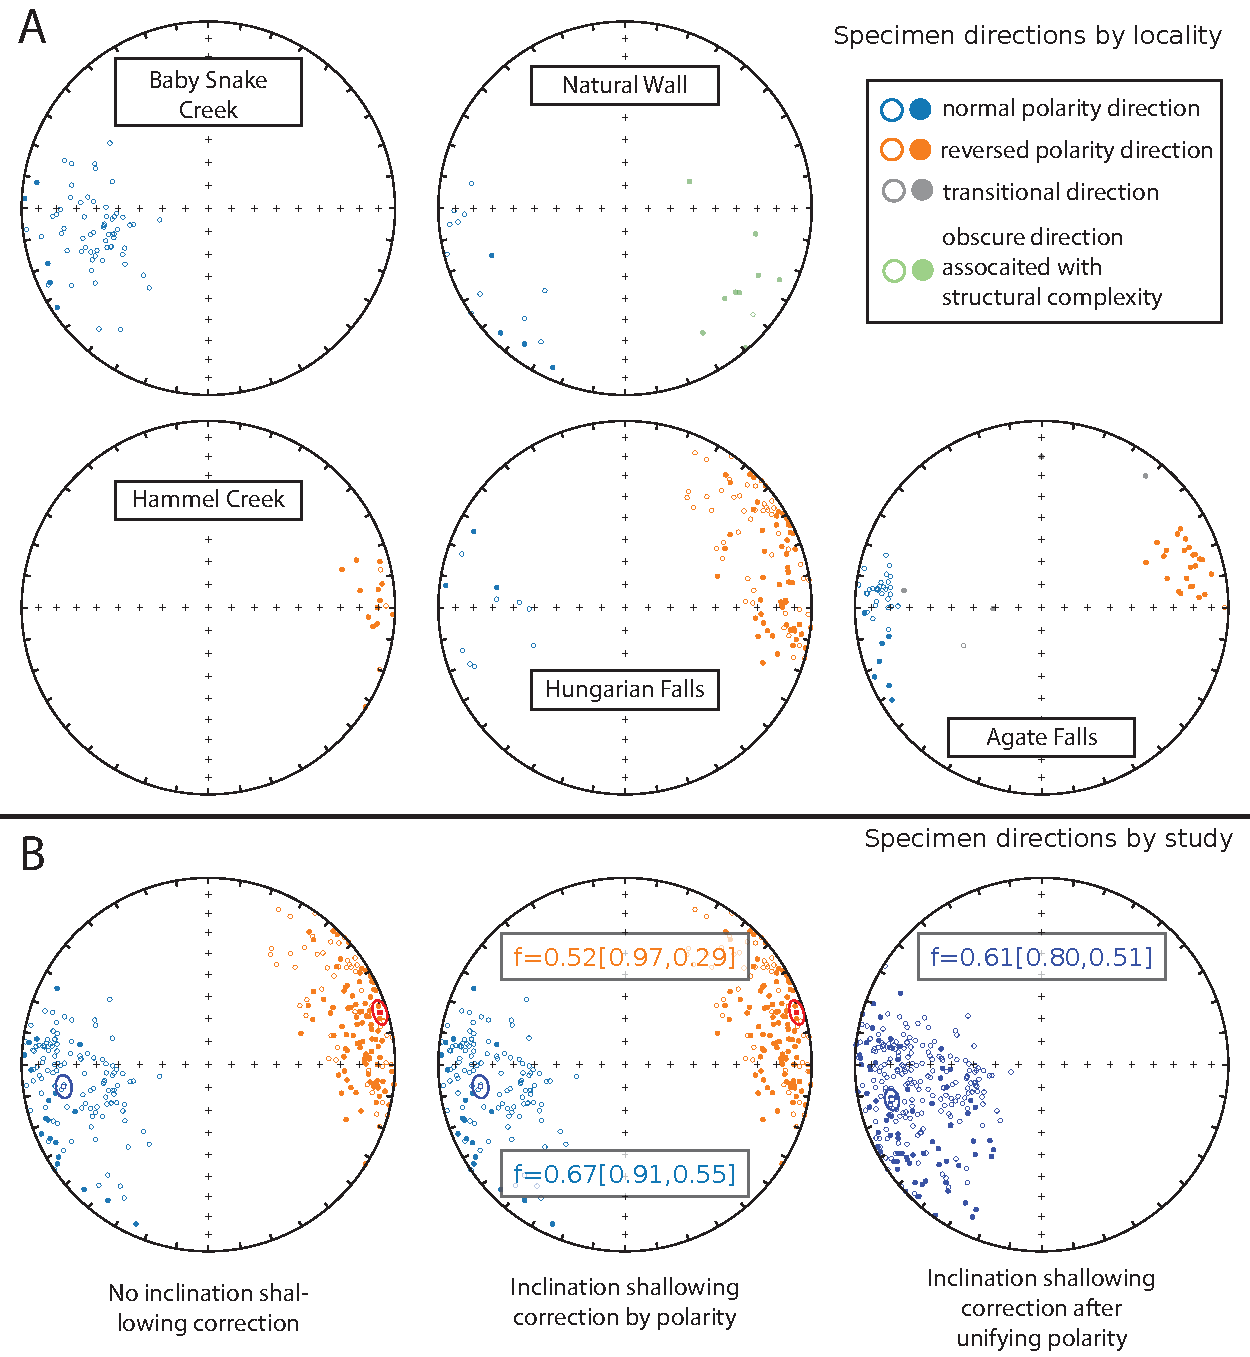
\includegraphics[width=\textwidth]{in_situ_pmag.pdf}
\caption{}
\label{fig:in_situ_pmag}
\end{figure*}

\begin{figure*}[h!]
\centering
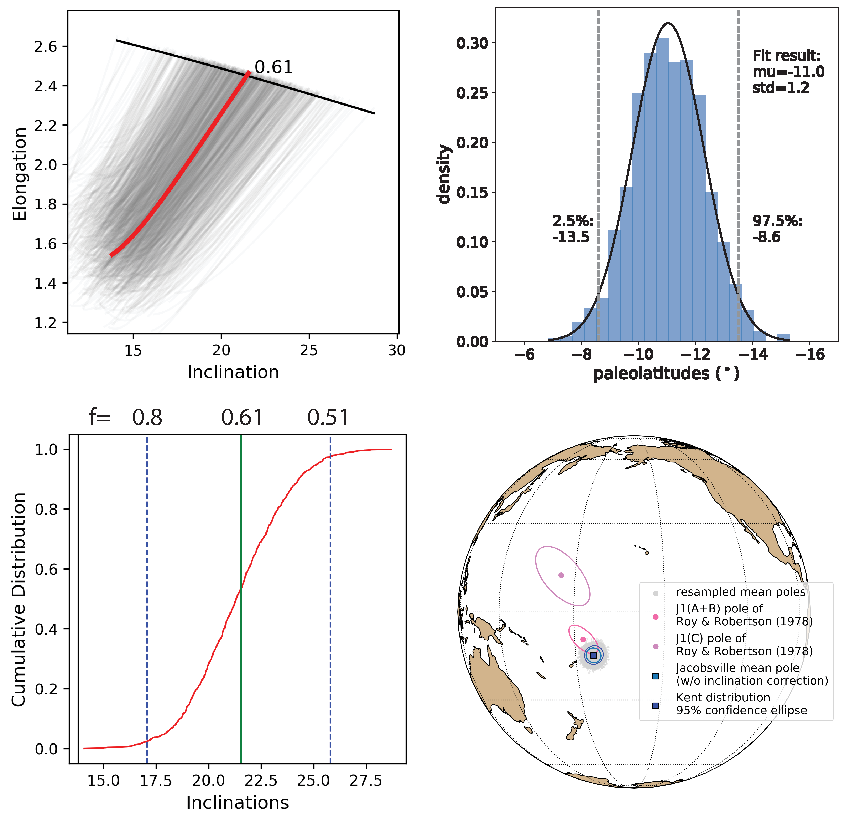
\includegraphics[width=\textwidth]{EI_results.pdf}
\caption{}
\label{fig:EI_results}
\end{figure*}

\begin{figure*}[h!]
\centering
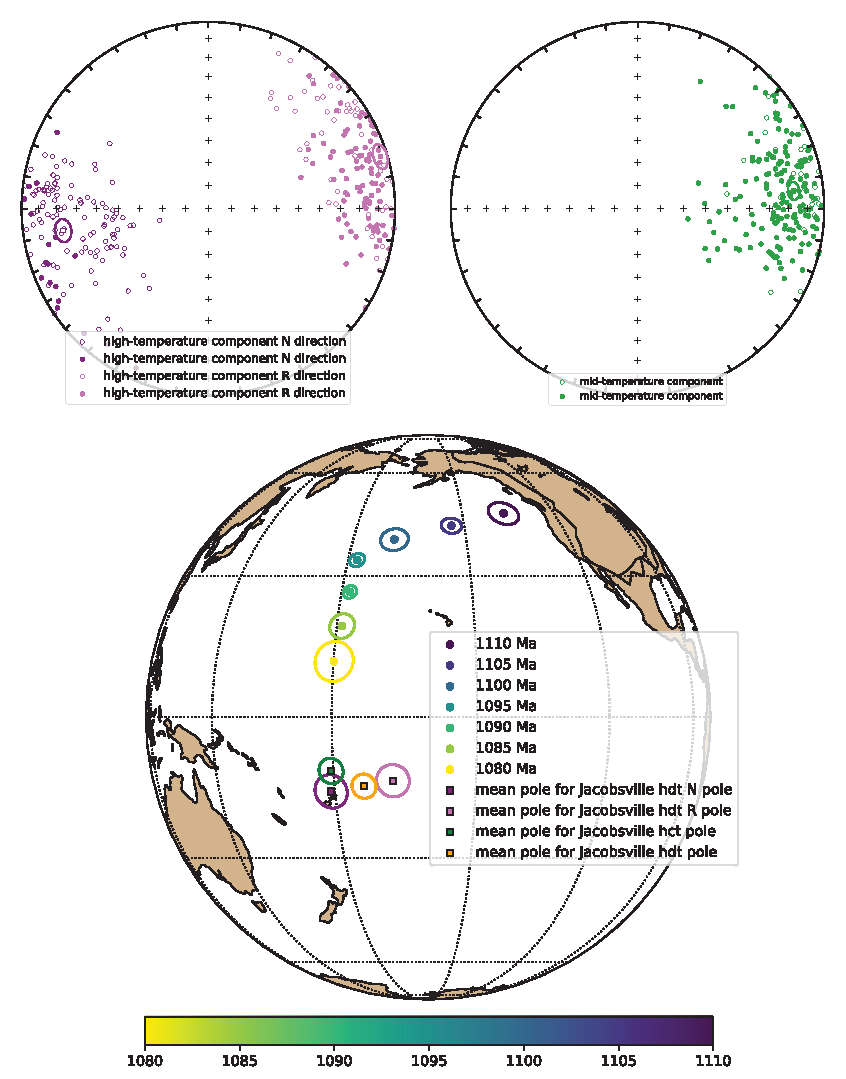
\includegraphics[width=\textwidth]{Jacobsville_pole_plot.pdf}
\caption{}
\label{fig:pole_plot}
\end{figure*}



\section*{Discussion}
\subsection*{Inclination shallowing correction and Jacobsville paleomagnetic pole}

Although igneous and sedimentary rocks associated with the North America Midcontinent Rift provided high-resolution record of the ca. 1110 to 1070 Ma Keweenawan Track which is the apparent polar wander path (APWP) for Laurentia in the Mesoproterozoic, high-quality paleogeographic constraints is lacking thereafter since tectonism in the interior of Laurentia entered a protracted period of quiescence until the emplacement of the ca. 780 Ma Gunbarrel large igneous province \cite{Harlan2003a}. The new paleomagnetic data developed from the Jacobsville Formation presents an opportunity to extend the Keweenawan Track toward the early Neoproterozoic as its maximum deposition age has been recently tightly constrained to be ca. 992 Ma \cite{Hodgin2022a}. 

However, inclination bias associated with sedimentary rocks need to be corrected when synthesizing a paleomagnetic pole. Rotation of ferromagnetic grains during sediment deposition and compaction during early diagenesis can result in the acquisition of a detrital remanent magnetization that is biased shallow relative to the local geomagnetic field in which it was acquired \cite{King1955a, Tauxe2005a, Kodama2012a}. This effect can be summarized as: 
\begin{equation*}
\textup{tan}(I_o) = f\textup{tan}(I_f)
\end{equation*}
where $f$ represents the amount of inclination shallowing, $I_o$ represents the observed inclination of the specimen magnetization and $I_f$ represents the inclination of the field in which the magnetization was acquired. If uncorrected, shallower inclinations obtained from sedimentary rocks can result in erroneously low estimates of paleolatitudes, biasing the interpreted past positions of continents and hindering plate reconstructions \cite{Domeier2012a}. Methods for correcting sedimentary inclination bias have been developed. They include laboratory-based measurements of magnetic mineral fabrics \cite<e.g.>{Kodama1992a, Bilardello2015a}, as well as statistical methods based on the evaluation of the deviation of virtual geomagnetic pole (VGP) distribution patterns recorded by sedimentary rocks with an assumed paleosecular variation model (the ``elongation/inclination" [E/I] method of \citeA{Tauxe2004b}). When a large number of sedimentary paleomagnetic samples (typically n$>$100) capture an extensive period of time such that the paleosecular variation is sufficiently averaged, the E/I method can give accurate estimates and is more efficient than lab-based methods. In the ca. 1.1 Ga Midcontinent Rift, \citeA{Pierce2022a} showed that the E/I method is effective in correcting the inclination bias recorded by the Cut Face Creek Sandstone---a lava flow-bracketed fluvial red bed sedimentary formation dominated by overbank deposition. 

Inclination shallowing is also present in the Jacobsville Formation. Scatter of the specimen high-temperature component directions in geographic coordinates show dispersion of declinations parallel to the bedding plane, indicating the directions are likely shallowed along the bedding-vertical plane (Fig. \ref{fig:in_situ_pmag}; \citeA{Tauxe2004b}). Since the deposition of the Jacobsville Formation span over geomagnetic field reversals, it is of interest to investigate the amount of inclination shallowing associated with the normal (n=130) and the reversed (n=148) polarity respectively. Applying the E/I method on the directions of normal polarity yields an estimated $f$ value of 0.67 with 95\% bootstrap uncertainty bounds from 0.91 to 0.55 (Fig. \ref{fig:in_situ_pmag}B). On the other hand, directions of reversed polarity yields an estimated $f$ factor of 0.52 with more uncertainties ranging from 0.97 to 0.29 (Fig. \ref{fig:in_situ_pmag}B). In addition, the dual-polarity directions do not pass a reversal test \cite{McFadden1990a, Tauxe2010a}, regardless of whether inclination correction is applied (Fig. \ref{fig:in_situ_pmag}). 

One interpretation of the polarity discrepancy could be that the deposition of the Jacobsville Formation was protracted such that the sediments at Hungarian Falls which dominantly record a reversed polarity was deposited prior to those at Baby Snake Creek which dominate the normal polarity records (Fig. \ref{fig:in_situ_pmag}). This is consistent with the magnetostratigraphic interpretation that Baby Snake Creek section is younger than the Hungarian Falls section (Fig. \ref{fig:strat_column}). Field observations of \citeA{Tyrrell2019a} and \citeA{Mueller2021a} near Bete Grise Bay, which is only $\sim$10 km east to Baby Snake Creek (Fig. \ref{fig:Geologic_map}), show that significant thrusting and deformation along the Keweenaw Fault and subsequent weathering of the Midcontinent Rift basalt occurred prior to the deposition of the Jacobsville Formation. In addition, U-Pb calcite geochronology and thermometry confirm that the final motion of $\sim$2 km of vertical displacement along the Keweenaw Fault occurred during the ca. 980 Ma Rigolet phase of the Grenvillian Orogeny and the majority of the Keweenaw Fault motion likely occurred much earlier during the ca. 1050 Ma Ottawan phase orogeny \cite{Hodgin2022b}. Therefore, we interpret that it is most likely that the Jacobsville Formation were deposited just prior to and during the Rigolet phase of the Grenvillian Orogeny with progressive sediment transportation to the northwest resulting in its onlapping on top of the volcanics in the northern tip of the Keweenaw Peninsula. As a result, the sediments at Baby Snake Creek records a slightly more southerly paleolatitude than those near Hungarian Falls as Laurentia's plate motion continues toward the south (Fig. \ref{fig:in_situ_pmag}, \ref{fig:pole_plot}). 

An alternative interpretation to the polarity discrepancy could be that there are insufficient samples such that either or both polarities are not average for secular variation. 


Overall, both inclination-corrected polarities recorded by the Jacobsville Formation show mean pole positions in the southern hemisphere with respect to today's continental configuration (normal polarity longitude=, latitude=, A95=; reversed polarity longitude= , latitude= , A95=). The two pole positions are close to each other, but are distinct from the youngest poles developed from rocks of the Midcontinent Rift (Fig. \ref{fig:pole_plot}). In addition, albeit that the Jacobsville sedimentation span over geomagnetic field reversals, the large arc distance between the poles of the Jacobsville Formation and that of the Freda Formation precludes the hypothesis that the Jacobsville Formation at the five studied localities (Fig. \ref{fig:Geologic_map}) is coeval with the Oronto Group and formed through a prolonged period of time. 

To succinctly summarize a paleomagnetic pole for the ca. 992 Ma Jacobsville Formation, we combine the directions of both polarities and reassess the amount of inclination shallowing of the combined directional dataset (Fig. \ref{fig:in_situ_pmag}). The resultant estimate for the $f$ value is 0.61, and the inclination-corrected mean direction is dec= , inc= , $\alpha_{95}$= . The bootstrap 95\% uncertainty range for the $f$ value range from 0.80 to 0.51, which overlaps with the uncertainty ranges of directions associated with each polarity (Fig. \ref{fig:in_situ_pmag}). The Fisher mean paleomagnetic pole associated with the combined directions is shown in Fig. \ref{fig:pole_plot} (pole longitude= 186.3\textdegree E, pole latitude= 14.3\textdegree S, A95= 2.5\textdegree). 

\citeA{Pierce2022a} discussed that as sedimentary grains usually flatten perpendicular to the bedding plane but circularly symmetric about the bedding plane, the resultant shallow inclinations they record would typically result in asymmetric uncertainties in the recorded paleomagnetic pole position with more uncertainties in paleolatitues than paleolongitudes. The asymmetric uncertainties associated with sedimentary paleomagnetic poles violate the assumption of a Fisher distribution \cite{Fisher1953a} where uncertainties associated with a mean pole position is circularly distributed. Instead, the spherical asymmetric bivariate Kent distribution \cite{Kent1983a} is more appropriate for incorporating uncertainties associated with inclination shallowing in reported sedimentary paleomagnetic poles. We follow the approach of \citeA{Pierce2022a} who extended the E/I method of \citeA{Tauxe2004b}. First we take all estimated $f$ values from the bootstrap results of the E/I algorithm and apply each value to correcting all Jacobsville detrital remanence directions. Then we calculate the Fisher statistics for each of the inclination-corrected mean poles. Finally we obtain 100 Monte Carlo resamples of each Fisher mean pole. As a result, the distribution of the resampled mean pole positions have an elongated distribution which represents more uncertainty associated with paleolatitudes of Laurentia than paleolongitudes (Fig. \ref{fig:pole_plot}). The distribution of paleolatitudes of the resampled mean poles can be well-approximated by a normal distribution (Fig. \ref{fig:pole_plot}). We use the Kent distribution to parameterize the 95\% confidence ellipse of the distribution of the resampled mean poles (mean longitude=186.4\textdegree E, mean latitude=14.2\textdegree S, major axis longitude=262.5, major axis latitude=43.5, major axis magnitude=3.3\textdegree, minor axis longitude=110.0, minor axis latitude=43.0, minor axis magnitude=3.0\textdegree; Fig. \ref{fig:pole_plot}). As is shown in Fig. \ref{fig:pole_plot}, although the Kent ellipse uncertainty range of the Jacobsville Formation's paleomagnetic pole position has significant overlap with the circular uncertainty range represented by the Fisher mean, the Kent ellipse informs more uncertainty along the great circle path between the mean pole position and the locality of the Jacobsville Formation as it incorporates the uncertainties in the amount of inclination shallowing within the sediments. 


% \subsection*{Age of the Grenville Loop}

\subsection*{Paleogeography of Laurentia during the late Mesoproterozoic to early Neoproterozoic}



\citeA{McCabe1983a} developed paleomagnetic data from the Chequamegan Sandstone of the Bayfield Group and found reversed-polarity directions similar to that of the Jacobsville Formation poles developed by \citeA{Roy1978a}. 




Although igneous paleomagnetic records from the the interior of Laurentia has been lacking since the end of the Midcontinent Rift magmatism, data from metamorphosed rocks associated with the ca. 1080 to 980 Ma Grenville continental collisional orogenesis has been developed to infer for Laurentia's plate configuration in the late Mesoproterozoic to early Neoproterozoic \cite<e.g.>{Weil1998a, Halls2015b}. However, in contrast to igneous rocks of the Midcontinent Rift which have relatively simple thermal history and straightforward paleomagnetic records \cite,e.g.>{Swanson-Hysell2019a}, rocks of the Grenville Province which experienced up to granulite facies metamorphism have much more complicated thermal history and the timing of their magnetic remanence acquisition is more difficult to constrain. As is shown in Fig. \ref{fig:pole_plot}, paleomagnetic poles developed from rocks of the Grenvillian Orogeny plots near Australia in today's continental reference frame, forming an arc distance of $\sim$30 degrees from the youngest paleomagnetic poles of the ca. 1070 Ma Freda Formation \cite{Henry1977a}. Such great discrepancies between pole positions associated with uncertainties in the age of the magnetization of the Grenville rocks led to the ``Grenville Problem" which is still highly debated today - did the Grenville rocks acquire magnetic remanence prior to the continental collision and thus the pole discrepancies are a result of significant crustal shortening (4000 $\pm$ 1000 km; \citeA<e.g.>{Halls2015b}), or did they acquire remanence after the continental accretion and thus the southerly poles merely represent Laurentia's continued motion through more recent times \cite<e.g.>{Weil1998a}?

As the ca. 990 Ma Jacobsville Formation was deposited in Laurentia Interior (Fig. \ref{fig:Geologic_map}), its paleomagnetic pole position can help test the contrasting hypothesis regarding the ``Grenville Problem". 





paleomagnetic mean pole of the Jacobsville Sandstone and the age

inclination shallowing correction of the Jacobsville Sandstone

magnetic reversal during the Jacobsville and the Maya Superchron

Implication on the crustal shortening of the Rigolet phase of the Grenville Orogeny

Warnock on the age of magnetization on the Haliburton pole: based on the very coarse thermal demagnetization steps Warnock2000a assigned that all of the primary magnetite components unblocked above 550 \textdegree C, with an uncertainty of 555 \textdegree C $\pm$ 5\textdegree C. Using a thermal history model that combines U-Pb titanite ages, hornblende and biotite Ar/Ar ages and just by merely compare the thermal history model with the assigned narrow magnetite unblocking temperature range, the authors assigned the age of the magnetization to be 1015 $\pm$ 15 Ma. 

It is important to note that the result Ar ages of the hornblende and biotite are 983 $\pm$ 8 Ma, 996 $\pm$ 8 Ma, and 998 $\pm$ 8 for hornblende with unblocking temperature of 530 $\pm$ 40\textdegree C, consistent across metamorphic terranes (Bancroft). And the biotite Ar ages are 910 $\pm$ 7 Ma, 891 $\pm$ 7 Ma, corresponding to unblocking temperature of 280 $\pm$ 40\textdegree C. 

More, the thermal demagnetization plots shown in Warnock2000a suggest that the magnetite unblocking lower temperature boundary can be around 500\textdegree C, lower than 555 $\pm$ 5\textdegree C. In addition, given the case that the rocks underwent uniform rate of cooling due to post-formation uplifting, a slow cooling effect from 555\textdegree C to 300\textdegree C from 990 Ma to 900 Ma allows for a scenario where the magnetite remament magnetization that appear to have a 555\textdegree C unblocking temperature in lab was acquired through a period of --- myr cooling though 500\textdegree C during uplifting. In this case, the magnetite remanence acquisition can be interpreted to be closer to the biotite Ar age than previously thought. Therefore, the Haliburton intrusion pole could be interpreted to be a post Rigolet orogenic activity phase magnetization acquisition, and the apparent discrepancy between the Haliburton pole and the Jacobsville pole can be explained by Laurentia's whole plate motion after the Grenvillian orogeny from 990 Ma to 900 Ma. One corollary of such scenario is that Laurentia underwent plate motion at a rate of ---\textdegree/myr, which is similar to that of today's tectonic plate motion. 

Crucial link between the Keweenawan Track and the Grenville Loop


\section*{Conclusion}



\acknowledgments
Enter acknowledgments, including your data availability statement, here.


\bibliography{YZ_ref}




\end{document}
